\documentclass[11pt,a4paper]{article}

\usepackage[margin=1in]{geometry}
\usepackage[T1]{fontenc}
\usepackage[utf8]{inputenc}
\usepackage{lmodern}
\usepackage{hyperref}
\usepackage{graphicx}
\usepackage{float}
\graphicspath{{report/figures/}{figures/}}

\hypersetup{
    colorlinks=true,
    linkcolor=black,
    citecolor=black,
    urlcolor=blue
}

\linespread{1.08}
\emergencystretch=2em

\title{\vspace{-1.5em}Proposal for Research Supervision:\\
Human-Centered Weather-Aware Travel Itinerary Optimization}
\author{[Your Name]}
\date{June 2026}

\begin{document}

\maketitle

\section*{Email Draft}

\noindent Subject: Request for supervision on a human-centered itinerary optimization project

\vspace{0.75em}

\noindent Dear Professor [Last Name],

\vspace{0.75em}

\noindent I hope you are doing well. I am writing to ask whether you might be open to supervising a research project that I am developing from my current weather-aware travel itinerary optimization system, with the goal of shaping it into a publishable HCI, recommender systems, spatial computing, or decision-support paper. I have one near-term HCI venue in mind as a possible target, but I am intentionally keeping the venue choice open until the contribution and evaluation design are clearer.

The current project began as an operations research and data science workflow for multi-day travel planning. It combines open-data enrichment, weather-aware congestion estimation, traveler preference modeling, mixed-integer route optimization, hotel/base-city selection, and interactive route visualization. The system currently supports profile-specific itineraries, nature-aware preference controls, route diversity, budget and time constraints, and map/dashboard exports. I would like to extend this technical prototype into a human-centered study of how people understand, trust, inspect, and adjust algorithmically generated travel plans under uncertainty.

The current repository is available as a \href{https://github.com/Ztang-Yit-Xiaang/weather-aware-travel-itinerary-optimization}{GitHub project}.

In the longer term, I hope to scale the system from regional scenarios to a nationwide travel-planning framework. My intended direction is to use lightweight agents at the beginning of the pipeline to help identify, fetch, and organize relevant datasets for a requested destination or region, while keeping the actual itinerary generation governed by explicit optimization methods rather than free-form generation. In other words, agents would support data acquisition and pipeline setup, but the route decisions would remain transparent, constraint-aware, and mathematically controlled.

I believe this project has publication potential because the core research question is not only whether the optimizer can produce feasible itineraries, but how an interactive decision-support system should communicate tradeoffs among weather risk, travel burden, attraction value, budget, pace, and personal interests. My tentative research framing is:

\begin{quote}
\emph{How can interactive itinerary planning systems help travelers negotiate uncertainty and tradeoffs while preserving agency over algorithmic recommendations?}
\end{quote}

\noindent I would especially value your guidance on turning the current system into a rigorous publishable contribution, including the research framing, user study design, evaluation metrics, and paper positioning. If an early-fall deadline is realistic, I would like to work toward it; if another venue is a better fit, I would also appreciate advice on how to adjust the scope and schedule.

\vspace{0.75em}

\noindent I have attached a short project proposal below. If this direction is potentially aligned with your interests, would you be available for a brief meeting to discuss whether it could be developed under your supervision?

\vspace{0.75em}

\noindent Thank you very much for considering my request.

\vspace{0.75em}

\noindent Best regards,\\
\mbox{[Your Name]}

\newpage

\section*{Short Project Proposal}

\subsection*{Working Title}

\noindent \textbf{Human-Centered Weather-Aware Travel Itinerary Optimization: Interactive Decision Support for Planning Under Contextual Uncertainty}

\subsection*{Potential Venues and Timeline}

\noindent A possible target is an HCI venue if the paper is framed around human-AI decision support, explanation, user agency, and empirical evaluation. One candidate is CHI 2027, whose full paper deadline is currently listed as September 10, 2026.\footnote{\url{https://chi2027.acm.org/authors/papers/}} However, I do not want to restrict the project to CHI too early. Depending on the supervisor's advice and the final contribution, other possible venue families could include intelligent user interfaces, recommender systems, geographic information systems, human-centered AI, visual analytics, or operations-research decision-support venues.

\subsection*{Project Background}

\noindent My current system treats travel planning as a constrained decision problem rather than a simple point-of-interest ranking task. It integrates:

\begin{itemize}
    \item attraction utility modeling from public rating and review signals;
    \item weather-aware congestion and waiting-time estimation using historical and forecast weather features;
    \item multi-day route optimization with attraction choice, visit sequencing, daily time limits, hotel/base-city decisions, travel-time penalties, and budget constraints;
    \item traveler profile controls for pace, such as relaxed, balanced, and explorer;
    \item an interest-profile layer that separates pace from preference, including nature, city, culture, and history weights;
    \item nature-aware planning for statewide and region-level trips, including national parks, scenic regions, gateway cities, detour costs, and weather exposure;
    \item interactive map and dashboard exports for route inspection and scenario comparison.
\end{itemize}

\noindent The current implementation is therefore a functioning technical substrate, with code and generated artifacts maintained in the \href{https://github.com/Ztang-Yit-Xiaang/weather-aware-travel-itinerary-optimization}{project repository}. However, to become a publishable research contribution, the next step is to study the human side of the system: how users make sense of recommended itineraries, how they revise them, which explanations matter, and where optimization-based planning supports or undermines user agency.

\subsection*{Long-Term Vision}

\noindent The future version of this project would expand beyond a single city or state-level demonstration toward a nationwide itinerary-planning system. A user could specify a broad region, such as a national park circuit, a multi-state road trip, or a city-plus-nature vacation, and the system would assemble the data needed for that planning context.

\noindent I am especially interested in a hybrid agent-plus-optimization architecture. At the beginning of the workflow, lightweight agents could help search for relevant public datasets, retrieve destination metadata, identify candidate attractions, collect weather and seasonal context, and prepare structured inputs for the model. However, the route itself would still be generated by formal optimization methods. This distinction is important: the agent would help with data discovery and preparation, while the optimization layer would preserve feasibility, interpretability, constraints, and reproducibility in the final itinerary.

\noindent This long-term direction also creates an HCI research opportunity. Users may need to understand not only why a route was selected, but also where the underlying data came from, what uncertainty exists in the retrieved data, and how much control they have over automated data collection versus route optimization.

\subsection*{Motivation}

\noindent Travel planning is a common high-stakes everyday decision: people spend time, money, vacation days, and emotional energy on plans that must remain feasible under changing weather, crowding, fatigue, transportation delays, and personal preferences. Many consumer itinerary tools emphasize attraction discovery or generated recommendations, but users often still need to reason manually about route feasibility, weather suitability, cost, and pacing.

This project asks whether a more transparent, interactive, and constraint-aware planning system can help users understand these tradeoffs. The research opportunity is to move beyond technical route quality and investigate the design of human-centered optimization interfaces: systems that do not simply output an ``optimal'' answer, but expose the consequences of different planning choices in a way that people can inspect, contest, and reshape.

\subsection*{Preliminary Research Questions}

\begin{enumerate}
    \item How do travelers understand and evaluate itinerary recommendations when the system explicitly shows tradeoffs among utility, weather risk, travel time, waiting time, budget, and interest fit?
    \item What kinds of explanations help users trust, question, or revise algorithmically generated travel plans?
    \item How should an interactive planning interface balance automated optimization with user agency and manual adjustment?
    \item Do preference controls such as pace profiles and interest bars help users express their planning intent more effectively than static recommendation filters?
\end{enumerate}

\subsection*{Proposed Contribution}

\noindent The intended paper could make four contributions:

\begin{enumerate}
    \item \textbf{A human-centered itinerary planning system} that combines weather-aware optimization with interactive preference control, route visualization, and explanation of selected and non-selected destinations.
    \item \textbf{A design and evaluation framework} for studying user interaction with optimization-based travel planning, especially under contextual uncertainty.
    \item \textbf{A hybrid agent-plus-optimization vision} in which agents assist with dataset discovery and preparation, while transparent optimization methods remain responsible for route generation.
    \item \textbf{Empirical findings} from a user study on how people interpret algorithmic travel recommendations, negotiate tradeoffs, and preserve agency when using a mixed predictive-prescriptive planning tool.
\end{enumerate}

\subsection*{Current Technical Foundation}

\noindent The prototype already includes the following components:

\begin{itemize}
    \item a Python package for itinerary system modules, including utility modeling, budget handling, data enrichment, region scenarios, route optimization, diversity, and map rendering;
    \item a Gurobi-based multi-day optimizer for attraction, hotel, and routing decisions;
    \item configurable trip scenarios through YAML files;
    \item support for nature-aware and city-aware preference profiles;
    \item validation scripts and tests for the pipeline;
    \item generated map and dashboard artifacts for inspecting selected routes and scenario outputs.
\end{itemize}

\noindent This foundation makes it possible to focus the publication work on interaction design, explanation, and empirical evaluation rather than beginning from a blank implementation.

\subsection*{Current Artifact Snapshot}

\noindent The current generated outputs make the project concrete enough to support a focused research study. The newest dashboard artifacts summarize a California Statewide Nature route, while the output tables compare route methods, trip lengths, city data quality, and interest profiles.

\begin{center}
\begin{tabular}{p{0.34\linewidth} p{0.56\linewidth}}
\hline
\textbf{Artifact} & \textbf{Current snapshot} \\
\hline
Candidate catalog & 228 candidate place records across seven California cities. \\
Default route method & Hierarchical + Bandit + Small Gurobi Repair. \\
Customer dashboard route & 7-day saved route artifact with 7 visible stops. \\
Method CSV snapshot & Hybrid repair method reports 16 selected attractions and approximately 2041.80 used from a 2213.14 buffered trip budget. \\
Trip-length comparison & 7-day, 9-day, and 12-day route artifacts are exported. \\
Dashboard route index & 32 route records: 7 customer-visible options and 25 research-only records. \\
Validation summary & The dashboard export validator passes, and the production map validation summary reports 97 PASS checks. \\
\hline
\end{tabular}
\end{center}

\subsection*{How the Current Tool Can Be Inspected}

\noindent The current prototype is intended to be viewed as a working research tool rather than only a mathematical model. The quickest inspection path is:

\begin{enumerate}
    \item clone or open the \href{https://github.com/Ztang-Yit-Xiaang/weather-aware-travel-itinerary-optimization}{GitHub repository};
    \item run \texttt{python scripts/serve\_dashboard.py};
    \item open the printed local URL for the full dashboard artifact;
    \item inspect \texttt{customer.html}, \texttt{research.html}, and \texttt{evaluation.html};
    \item compare the full dashboard with the lightweight share map artifact.
\end{enumerate}

\noindent The current dashboard folder is \texttt{results/figures/full\_interactive\_dashboard/}, and the share map path is \texttt{results/figures/lightweight\_share\_map.html}. This matters for the research framing because the system's contribution is not just route optimization. It also exposes the route as an inspectable artifact: selected hotels, customer-visible route controls, research/debug route layers, method comparisons, interest-profile variants, playback, active-stop explanations, and validation outputs can be reviewed by a human before the itinerary is trusted.

\subsection*{Prototype Screenshots}

\noindent The current prototype already produces browser-viewable route artifacts. Figure~\ref{fig:proposal-dashboard} shows the refreshed customer-mode dashboard with trip-length controls, interest presets, selected hotel context, weather preview, and map route labels. Figure~\ref{fig:proposal-share-map} shows the lightweight share map intended for quick communication of a selected route.

\begin{figure}[H]
\centering
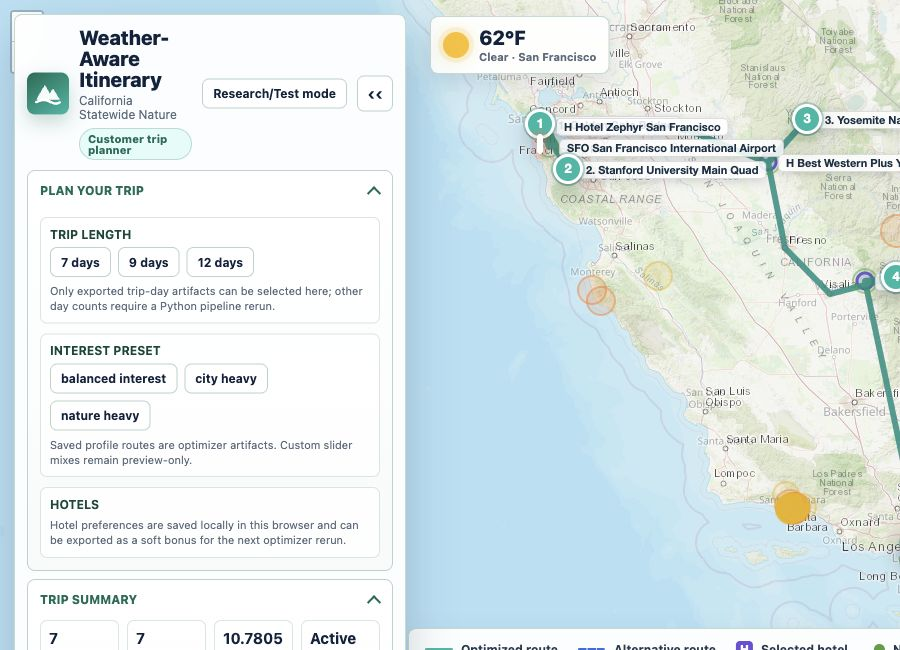
\includegraphics[width=0.92\linewidth]{figures/full_dashboard_screenshot.png}
\caption{Current customer-facing dashboard generated from the optimization pipeline.}
\label{fig:proposal-dashboard}
\end{figure}

\begin{figure}[H]
\centering
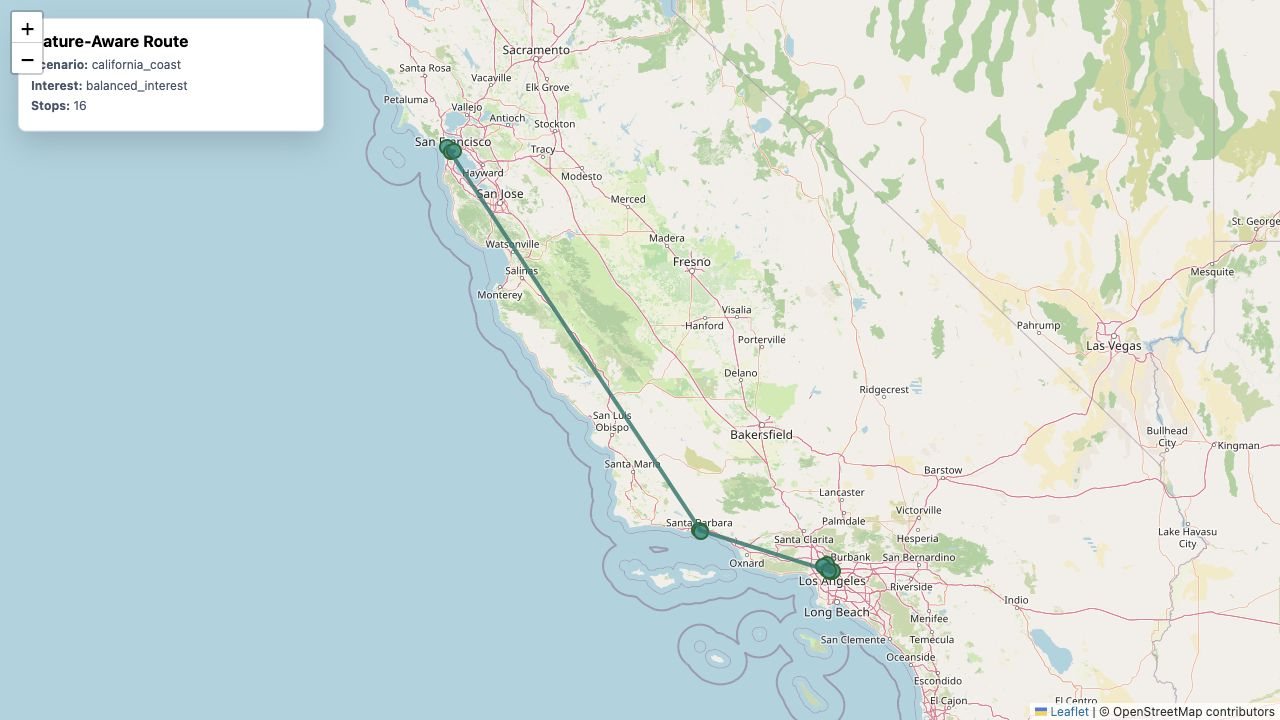
\includegraphics[width=0.92\linewidth]{figures/lightweight_share_map_screenshot.png}
\caption{Current lightweight share map showing a selected route artifact.}
\label{fig:proposal-share-map}
\end{figure}

\subsection*{Current Limitations}

\noindent The prototype is useful, but it should be described honestly:

\begin{itemize}
    \item The browser dashboard is a static export. It can switch saved route artifacts and show preview-only routes, but it does not rerun Gurobi in the browser.
    \item Some generated artifacts can become stale after configuration or code changes, so maps used as evidence should be regenerated before a paper submission.
    \item Live APIs may fall back to cached or curated data. This makes provenance and confidence reporting part of the research problem.
    \item Nationwide planning is a roadmap rather than a completed capability. The current strongest demo is California-focused.
    \item Waiting time and congestion are modeled through proxy signals, so the study should avoid overclaiming ground-truth crowd prediction.
    \item The evaluation dashboard should report solver statuses and fallback states directly so readers can distinguish exact optimization results from heuristic repairs.
\end{itemize}

\subsection*{Planned Research Design}

\noindent A feasible study plan could include:

\begin{enumerate}
    \item \textbf{Interface refinement.} Convert the existing dashboard into a study-ready interactive prototype where users can adjust interest weights, pace, budget, travel tolerance, and weather sensitivity, then inspect itinerary changes.
    \item \textbf{Scenario-based user study.} Ask participants to plan trips under different constraints, such as a sunny versus rainy forecast, relaxed versus ambitious pacing, or nature-heavy versus city-heavy preferences.
    \item \textbf{Comparison conditions.} Compare the proposed interactive optimization interface against a simpler ranked-list or static-map planning baseline.
    \item \textbf{Mixed-method evaluation.} Collect quantitative measures such as perceived control, trust, workload, plan satisfaction, and revision frequency, along with qualitative interview data about explanation usefulness and decision confidence.
\end{enumerate}

\subsection*{Expected Supervisor Guidance}

\noindent I am seeking supervision particularly on:

\begin{itemize}
    \item positioning the work within HCI, recommender systems, explainable AI, GIS/spatial computing, and human-centered optimization;
    \item narrowing the research questions to a publishable contribution;
    \item designing a rigorous and ethically appropriate user study;
    \item selecting suitable measures for trust, agency, workload, usability, and decision quality;
    \item recommending suitable publication venues and shaping the paper narrative for the chosen venue.
\end{itemize}

\subsection*{Proposed Work Plan}

\begin{center}
\begin{tabular}{p{0.22\linewidth} p{0.68\linewidth}}
\hline
\textbf{Period} & \textbf{Planned work} \\
\hline
June 2026 & Finalize research framing, related work map, study design, venue strategy, and interface requirements. \\
July 2026 & Build study-ready prototype, pilot tasks, refine explanations, prepare ethics/IRB materials if required. \\
August 2026 & Run pilot/user study, analyze quantitative and qualitative data, draft results and design implications. \\
Early September 2026 & If targeting CHI 2027, complete paper writing, figures, supplementary materials, anonymization, and submission package. \\
Fall 2026 onward & If another venue is a better fit, continue study refinement, paper revision, and submission preparation according to that venue's timeline. \\
\hline
\end{tabular}
\end{center}

\subsection*{Why This Is Publishable}

\noindent The project studies a socio-technical decision-support problem where algorithmic recommendations, user agency, uncertainty, explanation, spatial data quality, and interactive control are tightly connected. The technical system is not presented as the contribution by itself; rather, it enables an investigation into how people collaborate with optimization-based planning systems when real-world constraints and preferences conflict. CHI is one possible venue if the work is framed around human-AI interaction and empirical evaluation, but the project could also be positioned for venues centered on recommender systems, intelligent interfaces, geospatial computing, or optimization-based decision support.

\subsection*{Requested Next Step}

\noindent I would appreciate the opportunity to meet with Professor [Last Name] to discuss whether this project is suitable for supervision, how the contribution should be narrowed, which publication venue would be most appropriate, and what study design would be realistic for the next submission cycle.

\end{document}
